\chapter{Image Moments}
\label{ch:lesson05}

Once a blob can be isolated (Chapter~\ref{ch:lesson04}), \textbf{moments} let us summarize its shape with a handful of numbers: its area, centroid, orientation, and even a description that stays the same under translation, scale, and rotation. Moments offer a classic, lightweight alternative to learned features (covered in later chapters) for simple shape matching.

\section{What is a moment?}

For a binary image, the raw moment $m_{pq}$ is defined as
\begin{equation}
m_{pq} = \sum_{x,y} x^p\, y^q\, I(x,y),
\end{equation}
where $I(x,y)$ is 1 inside the shape and 0 elsewhere. A few special cases are already familiar quantities:
\begin{itemize}
  \item $m_{00}$ = area (pixel count)
  \item $(\bar x, \bar y) = (m_{10}/m_{00},\, m_{01}/m_{00})$ yields the centroid
\end{itemize}
The \textbf{order} of a moment is $p+q$: $m_{00}$ is zeroth-order, $m_{10}$ and $m_{01}$ are first-order, and $m_{20}$, $m_{11}$, $m_{02}$ are second-order.

The formula is just a weighted sum over pixel coordinates, so for a binary image it reduces to finding every foreground pixel's $(x, y)$ and summing $x^py^q$ over them:

\begin{lstlisting}
ys, xs = np.nonzero(im_tiny)   # (row, col) = (y, x) of every foreground pixel
m00 = len(xs)                  # area
m10 = xs.sum()                 # sum of x^1 y^0
m01 = ys.sum()                 # sum of x^0 y^1
# cv2.moments(im_tiny, binaryImage=True) agrees exactly with this hand computation
\end{lstlisting}

\section{An elongated, rotated blob}

To make orientation easy to eyeball and check against, draw a rotated ellipse.

\begin{notebox}
OpenCV's \code{cv2.ellipse} produces minor rendering artifacts around the border; the figures below instead use a hand-written scan-conversion (an explicit inside/outside test against the rotated-ellipse equation) for an exact, artifact-free shape. See the repository for the drawing routine.
\end{notebox}

\section{Area and centroid from moments}

\begin{lstlisting}
m = cv2.moments(im_binary, binaryImage=True)
area = m['m00']
cx, cy = m['m10'] / m['m00'], m['m01'] / m['m00']
\end{lstlisting}

Figure~\ref{fig:l05-1} marks the result on the ellipse.

\begin{figure}[h]
\centering
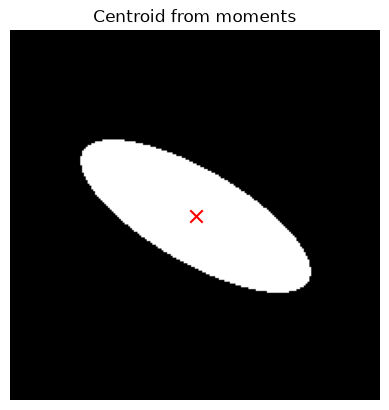
\includegraphics[width=0.4\textwidth]{figures/lesson05_fig03.png}
\caption{The centroid recovered from moments, marked on the rotated ellipse.}
\label{fig:l05-1}
\end{figure}

\section{Central moments}

Raw moments $m_{pq}$ depend on where the shape sits in the image --- move the shape and every $m_{ij}$ except $m_{00}$ changes. \textbf{Central moments} fix this by measuring around the shape's own centroid instead of the image origin:
\begin{equation}
\mu_{pq} = \sum_{x,y} (x-\bar x)^p\,(y-\bar y)^q\, I(x,y).
\end{equation}
Recomputing this sum from scratch would revisit every pixel again; instead, a shift-of-origin identity --- the image-moment analogue of the parallel-axis theorem --- gives, e.g., $\mu_{20} = m_{20} - \bar x\, m_{10}$, computed directly from the raw moments already in hand.

\section{Orientation from central moments}

The central moments $\mu_{20}$, $\mu_{02}$, $\mu_{11}$ describe the spread of the shape around its centroid --- essentially its covariance matrix (revisited in later chapters). The angle of the major axis (direction of greatest spread) is
\begin{equation}
\theta = \tfrac{1}{2}\,\operatorname{atan2}\bigl(2\mu_{11},\; \mu_{20}-\mu_{02}\bigr).
\end{equation}
The eigenvalues of the (normalized) covariance matrix built from $\mu_{20}, \mu_{11}, \mu_{02}$ give the axis lengths of the equivalent ellipse, plotted in Figure~\ref{fig:l05-2}.

\begin{figure}[h]
\centering
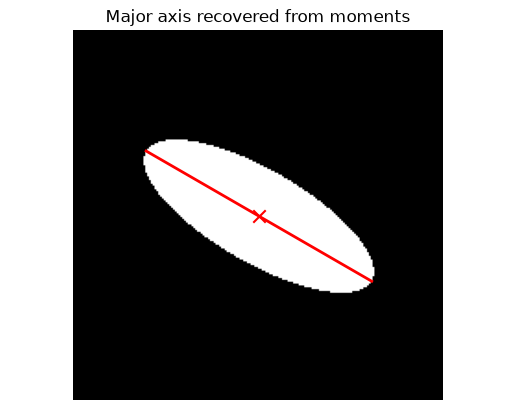
\includegraphics[width=0.4\textwidth]{figures/lesson05_fig04.png}
\caption{The major axis recovered purely from second-order central moments matches the ellipse's true drawn orientation.}
\label{fig:l05-2}
\end{figure}

\section{Hu moments: a shape descriptor invariant to pose}

\textbf{Hu moments} (\code{cv2.HuMoments}) are seven values calculated from the central moments that stay (nearly) the same regardless of the shape's position, size, and rotation --- useful for comparing two shapes without first aligning them. To test this, three versions of a dog silhouette (original, translated, and rotated $+$ scaled) are compared against each other and against a different shape (a cat silhouette), all shown in Figure~\ref{fig:l05-3}.

\begin{figure}[h]
\centering
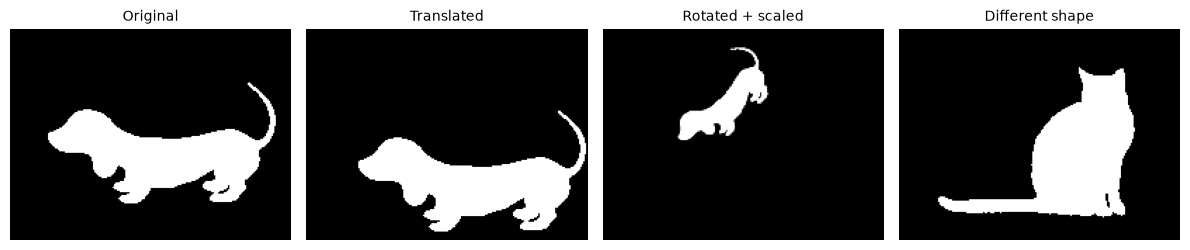
\includegraphics[width=0.95\textwidth]{figures/lesson05_fig05.png}
\caption{Original, translated, rotated $+$ scaled, and a different shape entirely. \attrib{Images: \href{https://www.publicdomainpictures.net}{Public Domain Pictures}.}}
\label{fig:l05-3}
\end{figure}

\begin{lstlisting}
def hu_log(im):
    m = cv2.moments(im, binaryImage=True)
    hu = cv2.HuMoments(m).flatten()
    return -np.sign(hu) * np.log10(np.abs(hu) + 1e-30)  # log-scale: raw values span many orders of magnitude
\end{lstlisting}

The translated and rotated+scaled versions yield similar (log-scaled) Hu moments to the original, whereas the different shape yields markedly different values --- exactly the invariance property that makes Hu moments useful for shape matching.

\subsection*{Exercises}
\begin{enumerate}
  \item Use \code{cv2.findContours} to get the outline of a blob from Chapter~\ref{ch:lesson04}'s binary image, then call \code{cv2.moments} on the \emph{contour} instead of the full binary mask. Compare the centroid to the one computed here.
  \item Draw a shape that is mirror-flipped rather than rotated. Are its Hu moments still close to the original? (Hint: think about what determinant/parity information moments do or do not capture.)
\end{enumerate}

\vfill
\fullcode{lesson05}{lesson05_moments}
